\documentclass[16pt,a4paper]{article}
\usepackage[utf8]{inputenc}
\usepackage[francais]{babel}
\usepackage[T1]{fontenc}
\usepackage{amsmath}
\usepackage{amsfonts}
\usepackage{amssymb}
\usepackage{graphicx}
\usepackage[final]{pdfpages} 
\author{Mory Ouattara}
\newcommand{\Nat}{\mathbb{N}}
\newcommand{\interp}[2]{\llbracket#1\rrbracket^{#2}}
\title{Master 1 Data-Science -INPHB }
\author{Analyse des données\\
Mory Ouattara}
\date{}
\begin{document}

%Les points sont donnés à titre indicatif.
\maketitle 
\thispagestyle{empty}

 \textbf{Exercice 1} \\
 
 On considère le tableau $K$ suivant où $a$ est un entier non nul :
 
  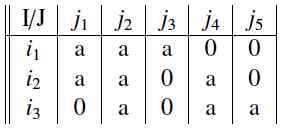
\includegraphics[scale=0.8]{SC1} 
  
  On pose : 

$I =\{i_1; i_2; i_3\}$ et $J = \{ j_1; j_2; j_3; j_4; j_5\}$

On effectue l'analyse factorielle des corresponsdances (AFC) de K.
 
 1-) Déterminer les centres de gravité des nuages $N(I)$ et $N(J)$
 
 2-) Déterminer la matrice des profils colonnes $F_1$ ainsi que la matrice des profils lignes $F_2$ de K.
 
 3-) Calculer le produit $F_1F_2$  
 
 4-) Quel est l’influence du réel $a$ sur l’AFC de ce tableau. 
 
 5-) Quel est l’axe factoriel trivial, à quelle valeur propre est-il associé ?
 
 6-) Quelle est l'inertie du nuage N(J).\\
 
 7-) On pose
  
  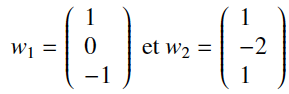
\includegraphics[scale=0.5]{SC2} 
  
 Montrer que $w_1$ et $w_2$ sont des vecteurs propres de $F_1F_2$, en déduire les axes factoriels non triviaux $u_1$ et $u_2$ ainsi que les valeurs propres associés. On choisira $u_1$ de manière
que la première coordonnée soit positive, de même pour $u_2$.
 
8-) Calculer $\varphi_\alpha(i)$ l'abscisse de la projection du profil de la ligne i sur le $\alpha$  avec la contrainte $\varphi_\alpha(i_1) \geq 0$


9-) Calculer  à l'aide des formules de transition,   $\psi_{\alpha}^j$ l’abscisse de la projection du profil de la colonne j sur le $\alpha$ ème axe factoriel.

10-) Représenter les deux nuages N(I) et N(J) simultanément dans le plan factoriel 1-2.

11-) Calculer la contribution de $i_1$ a chacun des axes factoriels non triviaux ainsi que la qualité de représentation de $i_1$ dans le plan factoriel 1-2 c’est-à-dire $COR1(i_1) + COR2(i_1)$.
 
\includepdf[pages=2]{PartAD.pdf}

\end{document}